\section{Cutting the profiling cost}

We use three heuristics to significantly reduce the profiling cost.


\subsection{Decoupling the decision knobs}
Instead of running an exhaustive search (which takes $O(n^k)$ 
in time to profile all configurations of $k$ knobs each having $n$ values), 
our first idea is to treat the knobs separately, and update each of their values 
while fixing the other knobs, so that we only run $n*k$ configurations. 
Policy~3 describes how we re-profile and update configurations by treating the
knobs separately. 

Policy~3 basically cuts the profiling cost by ignoring the interaction between knobs,
which could result in suboptimal configurations.
The insight behind this idea is that in video analytics, 
the resource-accuracy tradeoffs of configurations depend on mostly independent
aspects of videos, so the sweet-spot of the resource-accuracy tradeoff of a certain
knob is often independent to the value of other knobs.
For instance, the best frame sampling rate that strikes a balance between accuracy 
and resource depends on the speed of objects, while the best image size depends
on the size of the objects of interest. 

Formally, this can be described as following. 
Given two configurations $C_1$ and $C_2$ that share the same value $v$ 
on certain knob, suppose that the most expensive value of the knob is $v^*$, and
let $F(x,C,C\setminus\{v\}\cup \{v^*\})$ denote 
the accuracy of configuration $C$ 
on frame $x$, if substituting $v$ by $v^*$ in $C$ is the golden configuration.
\begin{align*}
    F(x,C_1,C_1\setminus\{v\}\cup \{v^*\})=
    F(x,C_2,C_2\setminus\{v\}\cup \{v^*\})
\end{align*}

This is consistent with our empirical results.
See Figure~\ref{fig:potential}

\begin{figure}
    \centering
    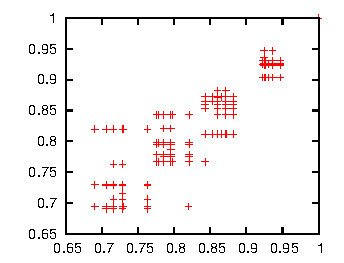
\includegraphics[width=0.25\textwidth]{figures/Profile_Sampling.pdf}
    \caption{X and Y axises are $F(x,C_1,C_1\setminus\{v\}\cup \{v^*\})$ and $F(x,C_2,C_2\setminus\{v\}\cup \{v^*\})$, respectively. Accuracy of the frame sampling rate is conditionally independent to 
    the values of other configuration knobs.}
    \label{fig:}
\end{figure}

\begin{figure}
    \centering
    \hspace{-0.5cm}
    \subfloat[Video clip \#1]
    {
        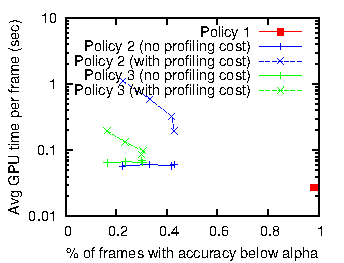
\includegraphics[width=0.4\textwidth]{figures/Bellevue_116th_NE12th_accThresh_80p_Comparison_Policy123.pdf}
        \label{subfig:1}
    }\\
    \subfloat[Video clip \#2]
    {
        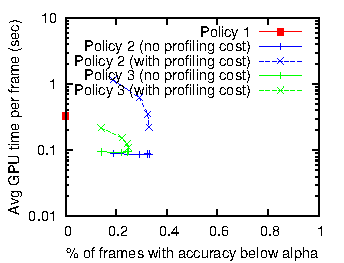
\includegraphics[width=0.4\textwidth]{figures/Bellevue_150th_Eastgate_accThresh_80p_Comparison_Policy123.pdf}
        \label{subfig:2}
    }
    \caption{}
    \label{fig:potential}
\end{figure}

\begin{policy}[Periodic Per-knob Search]
See Algorithm~\ref{alg:policy3}
\end{policy}

\begin{algorithm}
	\DontPrintSemicolon
	\KwIn{A list of frames in $t$ seconds ($t>n$), an accuracy threshold $\alpha$, and a set of potential values $V_k$ of each knob $k$ ($k=1,\dots,n$) of which the most expensive and cheapest value are $v_k^*$ and $v_k^'$ respectively}
    \KwOut{The best configuration $\hat{C}=(\hat{v_1},\dots,\hat{v_n})$}
    \tcc{\small{Set each knob to its cheapest value}}
    \ForEach{Knob $k$}{
        $\hat{v_k}\leftarrow v_k^'$
    }
    \tcc{\small{Optimize each knob separately}}
    \ForEach{Knob $k$}{
        $Resource_{min}\leftarrow$ Infinite\\
        $Accuracy_{best}\leftarrow 1$\\
        \ForEach{$v\in V_k$}{
            \tcc{\small{Computer the accuracy of using $v$ on knob $k$, while fixing other knobs}}
            $C(v)\leftarrow(\hat{v_1},\dots,v,\dots,\hat{v_n})$\\
            $Accuracy\leftarrow \frac{1}{|F|}\sum F(x,C(v),C(v)\setminus\{v\}\cup \{v_k^*\})$
            \If{$Resource(C(v)) < Resource_{min}$ and $Accuracy \geq \alpha$}{
                \tcc{\small{Set knob $k$ to $v$, if $v$ is cheaper and is accurate enough}}
                $\hat{v_k}\leftarrow v$\\
                $Resource_{min}\leftarrow Resource(C(v))$\\
                $Accuracy_{best}\leftarrow Accuracy$\\
            }
        }
        \tcc{\small{Update the accuracy threshold}}
        $\alpha=\frac{\alpha}{Accuracy_{best}}$
    }
    \Return{$\hat{C}\leftarrow(\hat{v_1},\dots,\hat{v_n})$}
	\caption{Policy 3: Periodic Per-knob Search}
	\label{alg:policy3}
\end{algorithm}



\subsection{Cross-camera inference}

\jc{TBD: (Spatial correlation) Further reduce the cost by amortizing the cost across similar cameras} 


\subsection{Smart triggering of update}

\jc{TBD: (Temporal correlation) Further reduce the cost by slowing down update if not ``change'' is detected} 